\documentclass{beamer}
\usepackage{booktabs}
\usepackage{bbding}
\usepackage{pdfpages}
\usepackage[absolute,overlay]{textpos}
\usepackage{amsmath}
\usepackage{graphicx}
\usepackage{tikz}
\usetikzlibrary{shadows}
\usetikzlibrary{shadows.blur}
\usetikzlibrary{patterns}
\usetikzlibrary{calc}
\usetheme[progressbar=foot,outer/numbering=none]{metropolis}           % Use metropolis theme

% https://github.com/matze/mtheme/issues/308
\usefonttheme{professionalfonts}
\usepackage{unicode-math}
\setmainfont{Fira Sans Light}  % Needs to be specified again!
\setmathfont{TeX Gyre Pagella Math}[Scale=MatchLowercase]  % Just a default
\setmathfont{Fira Sans Light}[range={up/{num,latin,Latin,greek,Greek},%
  \mathexclam,\mathplus,\pm,\div,\minus,\mathpercent,\mathampersand,%
  \mathquestion,\mathatsign,\increment,\less,\equal,\greater,\ne,\leq,%
  \geq,\matheth,\ell,\partial},%
  Script=Latin,script-features={}, sscript-features={}]
\setmathfont{Fira Sans Light Italic}[range={it/{latin,Latin,greek,Greek}},%
  Script=Latin, script-features={}, sscript-features={}]

\hypersetup{pdfauthor   = Jeongho Jeon,
            pdftitle    = Counterfactual: Generalized State Channels,
            pdfsubject  = Ethereum Sharding Research
            pdfkeywords = {counterfactual, ethereum, state channel},
            pdfproducer = LuaTeX 1.0.4,
            pdfcreator  = VIM 7.4}

\title{Counterfactual: Generalized State Channels}
\subtitle{Ethereum Sharding Research}
\date{July 23, 2018}
\author{Jeongho Jeon <maczniak@gmail.com>}
\institute{\textbf{Whitepaper} Foundation, Nonce\\%
(for internal discussion purposes only)}
\definecolor{boxbg}{HTML}{b4d4eb}
\definecolor{boxredish}{HTML}{ebb4d4}
\definecolor{boxlime}{HTML}{d4ebb4}
\usebackgroundtemplate%
{%
\begin{picture}(50,50)
\put(150,-232){\hbox{
\includegraphics[scale=0.1]{whitepaper_colored.png}}}
\end{picture}
}

\begin{document}

\maketitle

\begin{frame}{State/Payment Channel}
places as little on-chain as possible while still remaining secure.
\begin{description}
\item[Payment Channel] Lightning Network, Raiden, Teechain, eltoo, Sprites
\item[State Channel] Counterfactual, Perun, Pisa
\item[Application-specific Channel] Fate Channel (FunFair), Celer Network, Gnosis
\end{description}

$2/3$ sessions of Master workship: off the
 chain\footnote{https://github.com/state-of-blockchain-scalability/blockchain-conference-videos/blob/master/master-workshop-off-the-chain.md}
 (Jun 30-Jul 1) are related to state/payment channels.
\end{frame}

\begin{frame}{State/Payment Channel: Pros}
\begin{itemize}
\item the cheapest among scalability solutions
\item instant finalization upon participants' consent
\item fast withdrawal (e.g., cooperative withdrawal)
\item state channel network
\item (optional) partial choseout
\end{itemize}
\end{frame}

\begin{frame}{State/Payment Channel: Cons}
\begin{itemize}
\item participant availability (i.e., participants or delegates need to keep online.)
\item participants need to agree about currently finalized state quickly.
\item implement application-specific channels from scratch, without standard libiraries and reference implementations
\end{itemize}
\end{frame}

\begin{frame}{Comparison}
\fontsize{8}{9.6}\selectfont
\begin{tabular}{rccccc}
 & Lightning & Raiden & Sprites & Perun & Counterfactual \\
 \cmidrule(lr){2-2} \cmidrule(lr){3-3} \cmidrule(lr){4-4} \cmidrule(lr){5-5} \cmidrule(lr){6-6}
per payment path & \Checkmark & \Checkmark & \Checkmark & \Checkmark & \Checkmark \\
rent-a-path & & & \Checkmark & & \Checkmark \\
coop instant withdrawal & \Checkmark & & & & \Checkmark \\
partial closeout & \Checkmark & ? & ? & ? & \Checkmark \\
network setup & $O(n)$ & $O(n)$ & $O(1)$ & $O(\log n)$ & $O(1)$
\end{tabular}
\end{frame}

\begin{frame}{Counterfactual: Generalized State Channels}
%\begin{columns}
%\begin{column}{0.05\textwidth}\end{column}
%\begin{column}{0.50\textwidth}
\begin{minipage}{0.45\textwidth}
\fontsize{9}{10.8}\selectfont
\vspace{10pt}
released on Jun 12\footnote{https://twitter.com/statechannels/\\status/1006536423086977024a} by L4\footnote{https://l4.ventures/}, and updated on GitHub repository\footnote{https://github.com/counterfactual}.\\
``generalized'' means that participants can have only one state channel, and run a lot of applications parallelly on the channel.\\
Developers need not to know state channel details. It is designed with modular (code reuse) and open source style (no codes yet).
\end{minipage}
\begin{minipage}{0.40\textwidth}%
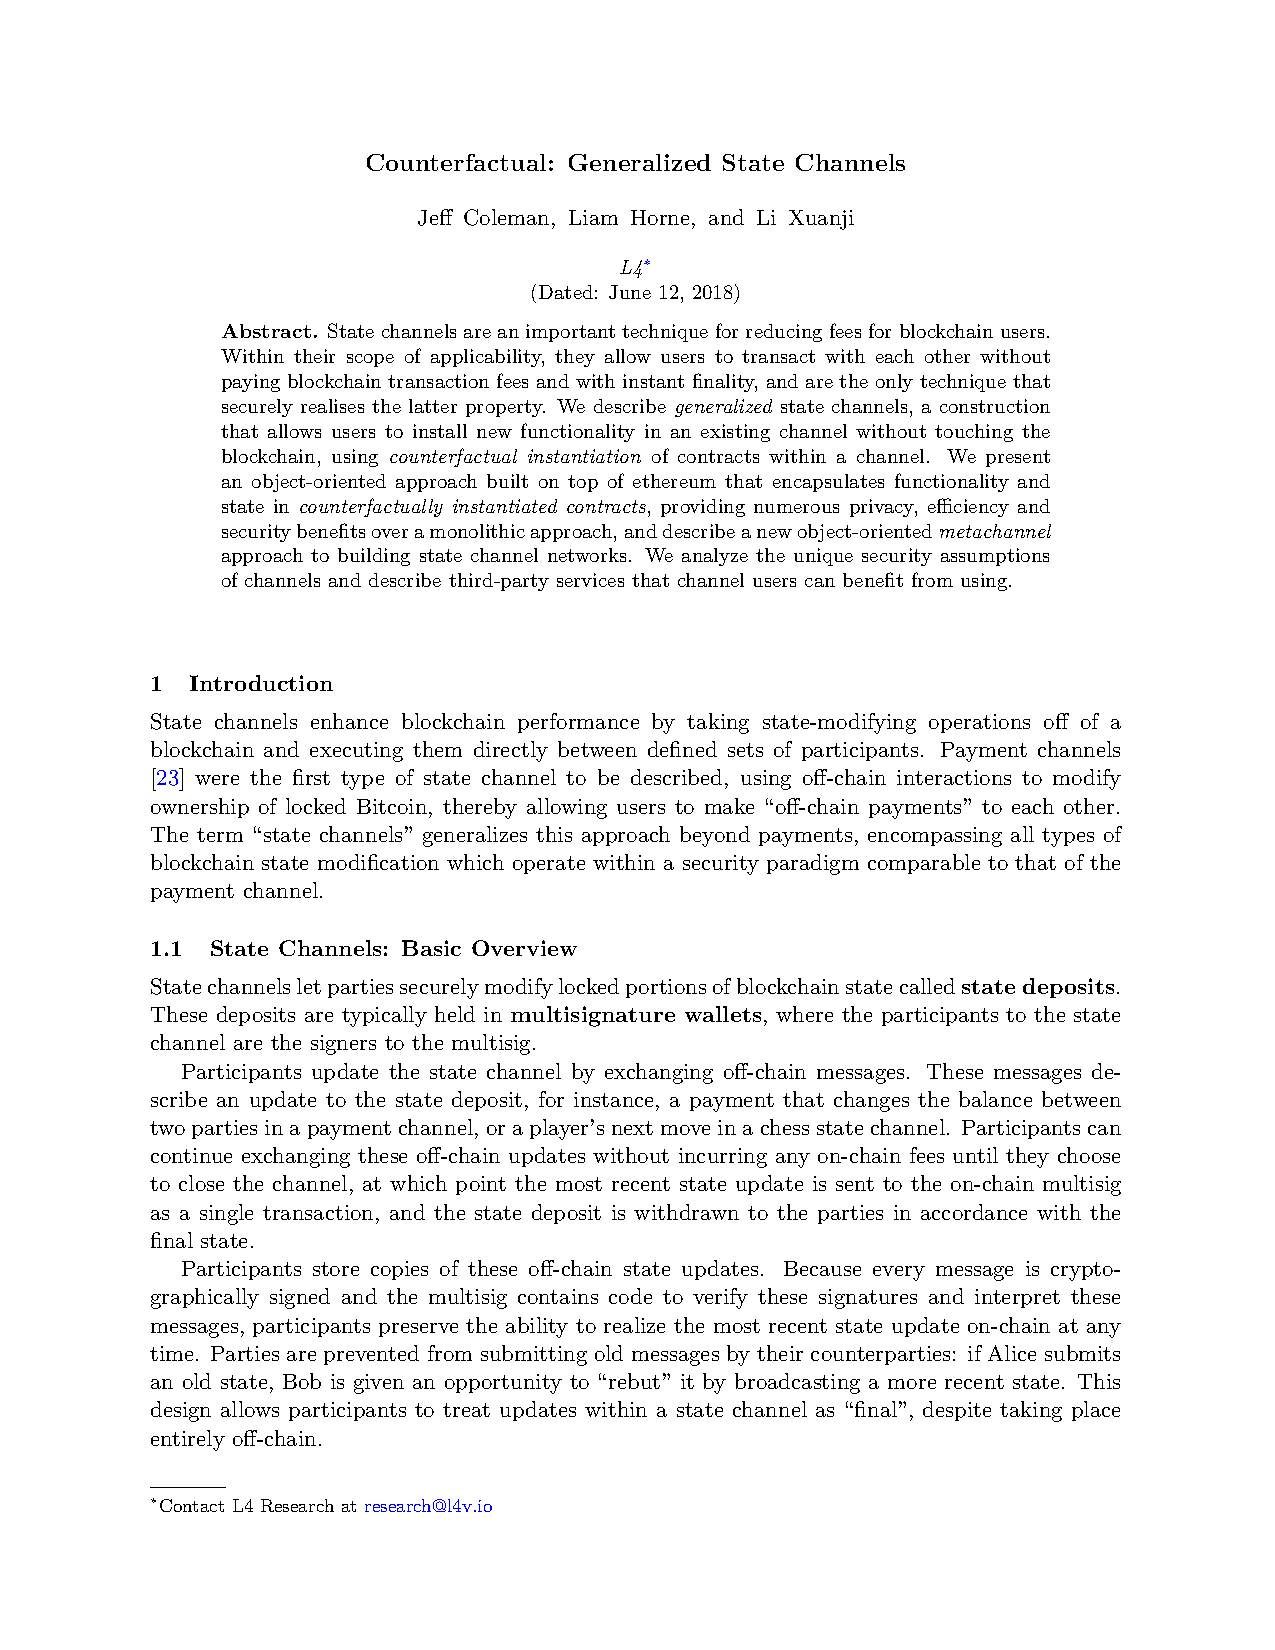
\includegraphics[page=1,scale=0.35,trim=-380 0 0 600]{statechannels.pdf}%
\end{minipage}
\end{frame}

\begin{frame}{counterfactual}
\begin{enumerate}
\item X could happen on-chain, but doesn’t
\item The enforcement mechanism allows any participant to unilaterally make X happen
\item Participants can act as though X has happened
\end{enumerate}
\end{frame}

\begin{frame}{counterfactual instantiation}
Counterfactual instantiation is the act of signing these commitments, not the act of actually calling deploy on-chain.\\
Counterfactual instantiation is the process by which members of a channel agree to be bound by an off-chain smart contract.\\
You can install and upgrade channel-based (channelized) applications without any on-chain operations (no fees).

Nonce-Dependent Conditional Finalization: The existence of state channel objects depends on nonce object's nonce.\\
All other objects depend on ``root nonce''.
\end{frame}

\begin{frame}{counterfactual address}
current contract address \texttt{sha3(rlp.encode([normalize\_address(sender), nonce]))[12:]}

counterfactual address of a contract need to be a deterministic function of the contract's initialization code. Ideas:
\begin{itemize}
\item ENS (Ethereum Name Service)
\item account abstract (depends on the code and a chosen salt)
\item skinny CREATE2 (endowment, memory\_start, memory\_length, salt) \texttt{sha3(msg.sender ++ salt ++ init\_code)[12:]}
\end{itemize}
\end{frame}

\begin{frame}{state}
Multisig wallets take control of state deposits.

Ethereum account state \texttt{(nonce, balance, contract code, storage)}

Counterfactual state is divided into nonce and application-specific state.
\end{frame}

\begin{frame}{Counterfactual Pros: Privacy}
Third party cannot tell state channels from multisig wallets.\\
Transaction details such as amount are visible only to participants.

\begin{quote}
A sufficiently powerful multisignature wallet is sufficient to act as a state deposit holder, and is the only on-chain component that must be deployed for each additional state channel.
\end{quote}
\end{frame}

\begin{frame}{Counterfactual metachannel}
\begin{itemize}
\item state channel network
\item not ``per payment path'' like Lightning $O(n)$ setup, but rent-a-path for a certain amount of time like Sprites $O(1)$ setup (that does not require cooperation from intermediaries for every payment)
\item onion routing - intermediaries cannot know the whole path
\end{itemize}
\end{frame}

\begin{frame}{Ideas}
\begin{itemize}
\item implement a (generalized) state channel
\item make a game on the top of the state channel
\end{itemize}
\end{frame}

\end{document}
